\documentclass[a4paper,10pt,openright]{memoir}

\setlength{\parindent}{0mm}

% Style of front page, title page, and stuff page
\usepackage{dikuReport}

% Not resetting figure counter on chapter
\usepackage{chngcntr}
\counterwithout{figure}{chapter}
\renewcommand\thefigure{\arabic{figure}} 



% Packages
\usepackage{listings}
\usepackage{minted}      % Syntax highlighting
%\usepackage{syntax}      % Used for writing grammars
\usepackage[all]{xy}
\usepackage{eucal}
\usepackage{enumerate}
\usepackage{hyperref}
\usepackage{wrapfig} % side captions on figures
\usepackage[justification=centering]{caption}
\usepackage{url}
\usepackage{mathptmx}
\usepackage{tabularx,colortbl}
\usepackage[normalem]{ulem}
\usepackage{soul}
\usepackage{eso-pic} % \AddToShipoutPicture
\usepackage{fancyhdr}
\usepackage{moreverb}
\usepackage{lscape}
\usepackage[stable]{footmisc}
\usepackage[latin1, utf8]{inputenc}
\usepackage{latexsym}
\usepackage[T1]{fontenc}
\usepackage{cite}
\usepackage{pdfpages}
\usepackage{tikz}
\usepackage{fix-cm}
\usepackage{xcolor,calc}
\usepackage{graphicx}
\usepackage{amsbsy}
\usepackage{amsfonts}
\usepackage{amssymb}
\usepackage{amsmath}
\usepackage{alltt}
\usepackage{float}
\usepackage{color}
\usepackage{relsize}
\usepackage{calc}
\usepackage{ifthen}
\usepackage{xspace}
\usepackage{caption}
\usepackage{lipsum}
\usepackage{listings}
\usepackage{color}
\usepackage{multicol}
\usepackage{xparse} % newDocumentCommand
\usepackage{enumitem}
\usepackage{csquotes}

%%%%% Make abbreviations emphasized.
\newcommand{\ie}{\emph{i.e.}\xspace}
\newcommand{\eg}{\emph{e.g.}\xspace}
\newcommand{\etc}{\emph{etc.}\xspace}
\newcommand{\vs}{\emph{vs.}\xspace}
\newcommand{\cf}{\emph{cf.}\xspace}
\newcommand{\viz}{\emph{viz.}\xspace}
\newcommand{\etal}{\emph{et~al.}\xspace}

%%% theorem commands
\newtheorem{definition}{Definition}[section]
\newtheorem{theorem}{Theorem}[section]

% Include some layout setup.
%!TEX root = main.tex

% NO RESETTING OF FOOTNOTES AT CHAPTER CHANGE
\usepackage{remreset}
\makeatletter\@removefromreset{footnote}{chapter}\makeatother

% Set the style of chapter heads

%\definecolor{TemplateColor}{rgb}{.75,.116,.60}  % KU Red
\definecolor{TemplateColor}{rgb}{.2941,.4549,.2359} % KU green

\newcommand{\pnumb}[1]{
    \begin{tikzpicture}
      \draw[fill,color=gray] (0,0) rectangle (5mm,5mm);
      \draw[color=white] (2.5mm,2.5mm) node { #1};
    \end{tikzpicture}
}    
\newcommand{\printchapternumm}{}
\makechapterstyle{combined}{
  \setlength{\midchapskip}{-60pt}
  \setlength{\afterchapskip}{2.5cm}
  \setlength{\parskip}{5mm}
  \renewcommand*{\printchaptername}{}
  \renewcommand*{\chapnumfont}{\normalfont\bfseries\fontsize{45}{0}\selectfont}
  \renewcommand*{\printchapternum}{\flushright\chapnumfont\textcolor{TemplateColor}{\thechapter}}
  \renewcommand*{\chaptitlefont}{\normalfont\Huge\bfseries}
  \renewcommand*{\printchaptertitle}[1]{%
    \raggedright\chaptitlefont\parbox[t]{\textwidth-2cm}{\raggedright##1}}
}

% Normal page numbering layout. How is always looks
\newcommand{\normalPN}{\makeevenfoot{plain}{}{\hspace{2mm}\thepage}{}\makeoddfoot{plain}{}{\thepage}{}}

% Special page numbering layout that is used for papers. Numbers are written in a gray box.
\newcommand{\specialPN}{\makeevenfoot{plain}{}{\\~\\~\\\hspace{2mm}\pnumb{\thepage}}{}\makeoddfoot{plain}{}{\\~\\~\\\pnumb{\thepage}}{}}

% Only clearpage (not cleardoublepage) at new chapter.
\renewcommand{\clearforchapter}{\clearpage}

\definecolor{codegreen}{rgb}{0,0.6,0}
\definecolor{codegray}{rgb}{0.5,0.5,0.5}
\definecolor{codepurple}{rgb}{0.58,0,0.82}
\definecolor{backcolour}{rgb}{0.95,0.95,0.92}
\captionsetup{labelfont=bf}

% Custom listing environment
\lstdefinestyle{mystyle}{
    backgroundcolor=\color{backcolour},   
    commentstyle=\color{codegreen},
    keywordstyle=\color{magenta},
    numberstyle=\tiny\color{codegray},
    stringstyle=\color{codepurple},
    basicstyle=\footnotesize,
    breakatwhitespace=false,         
    breaklines=true,                 
    captionpos=b,                    
    keepspaces=true,                 
    numbers=left,                    
    numbersep=5pt,                  
    showspaces=false,                
    showstringspaces=false,
    showtabs=false,                  
    tabsize=2
}

\lstdefinelanguage{Hermes}{
  keywords={call, uncall, printf, scanf, u32, u16, u8, true, false, if, for, \%u32},
  keywordstyle=\color{blue}\bfseries,
  ndkeywords={class, export, boolean, throw, implements, import, this},
  ndkeywordstyle=\color{darkgray}\bfseries,
  identifierstyle=\color{black},
  sensitive=false,
  comment=[l]{//},
  morecomment=[s]{/*}{*/},
  commentstyle=\color{codegreen}\ttfamily,
  stringstyle=\color{red}\ttfamily,
  morestring=[b]',
  morestring=[b]"
}

\lstdefinelanguage{ccustom}
{
morekeywords={of, and, fun, andalso, not, orelse, then, else, raise, let, in, end},
emph={SOME, NONE},
emphstyle={\color{teal}},
deletekeywords ={const, for},
sensitive=false,
morecomment=[l]{//},
morecomment=[s]{/*}{*/},
morecomment=[s]{(*}{*)},
morestring=[b]",
}

\lstset{style=mystyle, aboveskip=20pt,belowskip=20pt, xleftmargin=0.25cm, xrightmargin=0.25cm}

% Sets page numbering layout to normal
%\normalPN

% Where graphic files are located
\graphicspath{{Graphics/}}

% Alters the margins of the pages such that text are _not_ centered. This makes better room for the glue bindings.
\addtolength{\foremargin}{-35pt}
\addtolength{\spinemargin}{15pt}
\checkandfixthelayout

\setcounter{secnumdepth}{2}

% Basic information
\thesistype{Masters Thesis}
\thesiscomment{} % You can leave this blank
\title{Compiling a reversible lightweight cryptography language (Hermes) to assembly language ARM64 with focus on mitigating side-channel vulnerabilities}
\author{Hjalte Abelskov qdp218}
\supervisor{Michael Kirkedal Thomsen }
\date{February 28, 2019} % Hand-in date
\subject{Mitigating side channel vulnerabilities} % Short abstract not needed.
\begin{document}
\maketitle
\pagenumbering{roman}
\setcounter{page}{3}

% English Abstract
\cleardoublepage
\pagestyle{plain}
\begin{abstract}
english abstract
\end{abstract}

% Danish abstract
\clearpage
\begin{resume}
Dette speciale omhandler det reversible programmeringssprog Hermes, der er udviklet på DIKU som et domæne-specifikt sprog med henblik på implementatering af symmetriske krypteringsalgoritmer på små enheder.
Reversibiliteten i Hermes gør os i stand til at give nogle garantier for sikkerheden, idet visse side-kanal angreb såsom data-lækage bliver umuliggjort. Jeg beskriver disse side-kanaler samt reversibilitet og forklarer om intentionen om at sikre små enheder.
TODO: Jeg udvikler en ny ?backend? til Hermes, som skal forkorte antallet af trin i oversættelsen til mit valg af arkitektur, som er ARM64. Det vil give mere kontrol over side-kanaler idet vi ikke længere er afhængige af gcc og zerostack som bliver benyttet i den nuværende implementation af Hermes oversættelsen.
Min nye implementation er en to-trins process som først oversætter Hermes til et reversibelt statisk mellemliggende sprog med én tildeling af hver variabel (RSSA), der derfra kan oversættes til diverse arkitekturer - i dette tilfælde ARM64. Denne oversættelse fra RSSA til ARM64 udgør andet trin af oversættelsen.
Jeg implementerer 128-bit block cipheren Twofish og viser derved at Hermes er brugbart som et domæne-specifikt sprog til implementering af symmetriske krypteringsalgoritmer.
TODO: Til slut viser jeg korrektheden ved Twofish implementationen idet jeg anvender et eksisterende bibliotek til property based testing. 
TODO: Consider testing speed of 50 encryptions vs reference solution


\end{resume}

% Table of contents
\setcounter{tocdepth}{2} %Includes section, subsection and subsubsections in TOC
\cleardoublepage
\chapterstyle{combined}
\tableofcontents*

% Starting the real text.
\cleardoublepage
\pagenumbering{arabic}
\setcounter{page}{1}

\chapter{Introduction}
% Huffman, D.A.: Canonical forms for information-lossless finite-state logical machines.IRE Transactions on Information Theory5(5), 41–59 (1959)  First reversible computing guy
%Problemet med sidekanaler (skal lede op til baggrundsafsnittet)
%Nævn evt. også noget om små devices.

% Motivation
While our conventional cryptography methods, such as AES (encryption), SHA-256 (hashing) and RSA/Elliptic Curve (signing) work well on systems with reasonable processing power and memory capabilities, these do not scale well into a world with embedded systems and sensor networks.
This introduces some challenges such as how to reduce the amount of costly operations whilst still guaranteeing the highest level of security. The limits related to physical size, processing power, memory and battery life call for more lightweight cryptography methods to be implemented on such systems.
Lightweight cryptography applications can be implemented in many programming languages, most of which still leave the devices open to more sophisticated hacking methods such as timing attacks. These side-channel vulnerabilities are, at least in theory, avoidable if we choose our language of implementation carefully.

\section{Reversible Programming}
% NAND gates are irreversible.
% Landaurs principle is that heat must be generated when doing any "logically irreversible manipulation of information".

Reversible programming is a programming paradigm dating back to the early 1960s. Gordon Moore, the CEO of Intel, whose paper from 1965 describes a doubling of the number of transistors in a computers approximately every 18 months has led many people to believe that computing power would also double roughly every two years. This has been largely true until now, but as Rolf Landaur argues: this is ultimately going to come to an end due to overheating problems.
He argued that any irreversible operation must result in some kind of heat dissipation and that theoretically, with reversible operations, if operation A pushes the machine from an original state into some new state, then operation A$^{-1}$ could use the already existing energy in the system to push it back to the original state.
Such a machine has not yet been invented, but reversible programming has other interesting properties.
As discussed in section \ref{chapt - Reversible-computing}, it can serve as protection against side-channel attacks and is also an interesting field to study to better understand quantum computing.

\section{Basis for the work}
This goal of this thesis is to further extend Hermes, which is a reversible programming language developed at DIKU.
Hermes is based on the reversible programming language Janus and designed specifically for writing encryption algorithms [5].
By virtue of some carefully thought-out design choices, Hermes offers a built-in protection against some side-channel attacks.

In the current implementation, Hermes programs are translated to C by the program \emph{hc} and then to assembly code with the GNU Compiler Collection (gcc). The gcc compiler does not prevent side-channel attacks per default, but one can use zerostack [1] to zero out the stack and registers of sensitive functions.
There is also the problem of timing attacks introduced by gcc [2].
This compilation from Hermes to assembly is a two-step process with a required extra check by zerostack. But with embedded systems being the focus of these reversible lightweight cryptography algorithms, it seems appropriate with a compiler that translates Hermes directly to ARM assembly code.


%[1] \href{https://github.com/lmrs2/zerostack}{zerostack: Zeroing stack and registers of sensitive functions. Github project by lmrs2} \\
%
%\noindent [2] \href{https://drive.google.com/file/d/1jsOolD1C\_Fu9oNVvhkB1\_RQ9GlrFSGcN}{David Chisnall, Laurent Simon, Ross Anderson. What you get is what you C: Controlling side effects in mainstream C compilers} \\
%
%\noindent [3] Chris Lutz, Howard Derby. B. Parser, and JANUS Language Syntax JANUS : A TIME-REVERSIBLE LANGUAGE A . Lexical Analyzer. pages 1–4, 1986. \\
%
%\noindent [4] Tetsuo Yokoyama, Holger Bock Axelsen, and Robert Glück. Principles of a reversible programming language. In Proceedings of the 2008 conference on Computing frontiers - CF ’08, 2008. \\
%
%\noindent [5] Torben Ægidius Mogensen. Hermes: A Language for Writing Encryption Algorithms.

\input{Sections/Introduction/Related_Works.tex}
\section{Outline}
This thesis is organized as follows: section 2 introduces reversibility, side-channel vulnerabilities, the ARM architecture and RSSA. Section 3 analyzes how to compile from Hermes to ARM whilst mitigating side-channels and goes over the parts of ARM we need for the translation. Section 4 covers the compilation. Section 5 concerns the symmetric encryption algorithm Twofish and my Hermes implementation of it. Section 6 is about benchmarks and testing. Section 7 is a discussion of the results and finally in Section 8 I present my conclusions and ideas for future work.


% Baggrund om reversible computing og twofish algoritmen (referer til michaels artikel om reversibel symmetrisk krypto)
\chapter{The Concept of Reversible Computing}
\label{chapt - Concept of reversible computing}
% Skal bruge: Principles of a reversible programming language - Tetsuo, holger bock, robert gluck
%             Partial evaluation of the reversible language Janus - Torben M.
%             Encryption and reversible computations - dominik taborsky, Ken F.L, Michael
%             Reversible computation and reversible PL - Tetsuo
%             TODO: A reversible programming language and its invertible self-interpreter - Yokoyama, robert gluck
%             TODO: Hermes: A reversible language for writing encryption algorithms - Torben MogensenReversible computing is an interesting paradigm with regards to security. In reversible computing one writes programs in reversible programming languages such as Janus [3].

Reversible programs can be run both forwards and backwards deterministically, calculating output from input as well as input from output [4].
What this means is that all functions are bidirectional, i.e. given some resulting output of a function, we can run the inverse of that function with the output and find the initial input.
This is especially useful for algorithms, such as encryption or encoding, where an inverse process is most often needed.
If implemented without too much overhead, this will result in smaller programs, as the encoding/encryption function is bidirectional and can be used for decoding/decryption as well.

Being bidirectional imposes some constraints on the programmer: variables local to a function must be initialized to zero and reset to zero after use.
All variable updates must be lossless, therefore not allowing modulo updates such as \textbf{x = x mod y} as there is no inverse to this operation.
Bit-shift operations must also be lossless, i.e. when bits are rotated off the right end they are inserted into the vacated bit positions on the left and vice-versa. While imposing some restrictions on the programmer, reversible programming languages has a lot to offer in terms of security: they ensure no loss of information, as all variables are cleared after use. Thus the memory will not contain any data that can be used for side-channel attacks such as information leakage.

% Landaur embedding is embedding functions inside a larger function that we can then uncall
% Allows for irreversibility but makes the computer more of a lookup table than an actual computer
% We get around this by only allowing logically reversible computations

% Bennet embedding is what we want to use?

\section{Embeddings and heat dissipation}
Another motivation for researching reversible computing is heat dissipation; current transitor-based computing devices dissipate energy as heat and cooling of computational devices has become the main focus for the semiconductor industry \cite{semiconductors_valley}. In 1961 R. Landaur suggested reversible computing could be a way to minimize energy dissipation from a system \cite{Irreversibility_paper}.
Similar to how kinetic and potential energy work, computing a result would put the machine in a state with some energy that would enable it to invert the computation.
Landaur also proposed a way to make irreversible programs reversible. We call this the Landaur embedding.
%Most languages are not reversible, because they throw away information about the computers history, making it ambigious to find the predecessor state. 

%Logic reversibility implies that information is conserved and most languages are not backwards deterministic because some of their operations are logically irreversible and throw away information about the computers history, making it ambiguous to find the predecessor state.
%Embeddings are a way to make an irreversible computer reversible.

\subsection{Landaur embedding}
What Landaur saw was that any logically irreversible program could be transformed into a reversible one by wrapping it in a larger program with extra parameters that could hold any information needed for reversability. He proposed that the computer could have an extra tape where it would save all of its computation history. That way it would know how to run in reverse. But the size of saving this computation history is proportional to the execution time of the program.

Based on the idea that computation is cheap and erasure of data is expensive, Landaur's Embedding is not very efficient since it merely postpones the inevitable erasure of information when the tape needs to be cleared before the next computation.
Landaur demonstrated that whenever a computer throws away information about its previous state it results in a heat dissipation of $kT ln 2$ for each bit of information lost.
\subsection{Bennett embedding}
In 1973 C.H. Bennett came up with a new embedding that would turn out to be much more useful\cite{Bennett1973LogicalRO}.
The idea is that the machine can use the inverse of its transition function to carry out the entire computation backwards, completely resetting the history tape to its original blank state by computation. One only needs to copy over the output once it has been calculated before starting the cleanup. This way the data is reset through computation instead of erasure, which in theory should be much cheaper.
It uses three tapes: one for the forwards/backwards calculation, one for computation history and a third for copying over the output. 
In theory, this reduces the energy dissipated by roughly a factor ten.

\section{Reversibility in Hermes}
% We do not overwrite data in Hermes until we have set it back to 0 at the end of the function?
Hermes is a reversible programming language designed for encryption algorithms. It offers forwards determinism as well as backwards determinism its calculations, meaning that nomatter if it executes forwards or backwards,  there is only one possible state that the machine can transition to nomatter what state it is currently in.
This results in a one-to-one relationship between input and output states that is achieved through reversible updates, swaps and so on.
% Hermes uses pass-by-reference, so no global variables.
Hermes and its predecessor Janus uses pass-by-reference, which is where every argument passed to a function is a direct reference to the variable.
This imposes certain restrictions on parameter passing: there has to be the same amount of parameters for a call / uncall of a function as these are implicitly both the input and output of a function.
There can be no global variables and no variable can be passed to a function multiple times e.g. \emph{foo(x, x, y)}.
Furthermore, an alias on both sides of an update such as \textbf{x += x / y} can break reversibility.

% Show Hermes grammar?
\subsection{Grammar}
The grammar of Hermes is as follows:
\begin{figure}[htp]
\centering
\begin{tabular}{>{$}l<{$}>{$}r<{$}>{$}l<{$}}
    Program   & \rightarrow & Procedure^+ \\[7pt]
    Procedure & \rightarrow & \textbf{id} \; ( \; Decls2^? \; ) \; Stmt \\[7pt]
    Stmt      & \rightarrow &; \\
              & |           & Lval \; \textbf{update} \; Exp \;; \\
              & |           & Lval\text{++} \;; \\
              & |           & Lval\text{- -} \;; \\
              & |           & \texttt{if} \; ( \; Exp \; ) \; Lval \; \textbf{update} \; Exp \;; \\
              & |           & Lval \; \text{<->} \; Lval \;; \\
              & |           & \texttt{if} \; ( \; Exp \; ) \; Lval \; \text{<->} \; Exp \;; \\
              & |           & \texttt{for} \; ( \; \textbf{id} = Exp \; ; \; Exp \; ) \; Stmt  \;; \\
              & |           & \texttt{assert} \; ( \; Exp \; ) \;; \\
              & |           & \texttt{call} \; \textbf{id} \; ( \; Lvals \; ) \;; \\
              & |           & \texttt{uncall} \; \textbf{id} \; ( \; Lvals \; ) \;; \\
              & |           & \texttt{printf} \; ( \; \textbf{stringConst} \; , \; Lvals \; ) \;; \\
              & |           & \texttt{scanf} \; ( \; \textbf{stringConst} \; , \; Lvals \; ) \;; \\
              & |           & \{ \; Decls1 \; Stmt^* \; \} \\[7pt]
    Exp       & \rightarrow & Lval \\
              & |           & \textbf{numConst} \; \\
              & |           & Exp \; \textbf{binOp} \; Exp \\
              & |           & \textbf{unOp} \; Exp \\
              & |           & ( \; Exp \; ) \; \\[7pt]
    Lval      & \rightarrow & \textbf{id}\\
              & |           & \textbf{id} \; [ \; Exp \; ] \\[7pt]
    Lvals     & \rightarrow & Lval \\
              & |           & Lval \; , \; Lvals \\[7pt]
    VarSpec   & \rightarrow & \textbf{id}\\
              & |           & \textbf{id} \; [ \; \textbf{numConst} \; ] \\[7pt]
    VarSpecs  & \rightarrow & VarSpec \\
              & |           & VarSpec \; , \; VarSpecs \\[7pt]
    Decls1    & \rightarrow & \\
              & |           & \textbf{type} \; Varspecs \; ; \; Decls1\\
              & |           & \texttt{const}\;\textbf{type}\;\textbf{id}\;=\textbf{numConst}\;;\;Decls1\;\\[7pt]
    Decls2    & \rightarrow & \textbf{type} \; VarSpec \\
              & |           &  \textbf{type} \; VarSpec \; , \; Decls2

\end{tabular}
\caption{Grammar of Hermes.}
\label{fig: grammar}
\end{figure}



% Show control flows?
\subsection{Control flows}
Unlike most other programming languages (including Janus), Hermes does not have branching. It has two special types of if-statements being the conditional update and conditional swap. These conditionals only allow for one line of code to be executed, i.e. the swap or the update, and have a constant execution time. This is because they are constructed in such a way that the code of the conditional is always evaluated but only takes effect or gets executed if the condition is true.
Conditionals work on integers, which with the help of a logical AND, allows the update to only update in cases where the conditional is non-zero, i.e. true. As seen from figure ~\ref{fig:conditionals_c}, the conditional \textbf{(0 != a < 2)} with a minus in front either returns 0 or -1, which as a signed bit-representation is all ones, meaning that whatever you AND will remain in the result. This makes the update take effect. Had the conditional been 0, the AND operation would have resulted in bits being 0, which would have turned the expression into \textbf{x += 0}.
Swap is done with three XOR operations, which ensures reversability and does not introduce any extra temporary variables.
\begin{figure}
    \centering
    \begin{minipage}{0.35\textwidth}
        \centering
        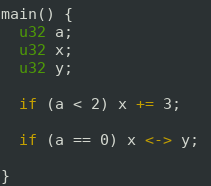
\includegraphics[width=0.9\textwidth]{conditionals_hms.png}
        \caption{Conditionals in Hermes}
    \end{minipage}\hfill
    \begin{minipage}{0.60\textwidth}
        \centering
        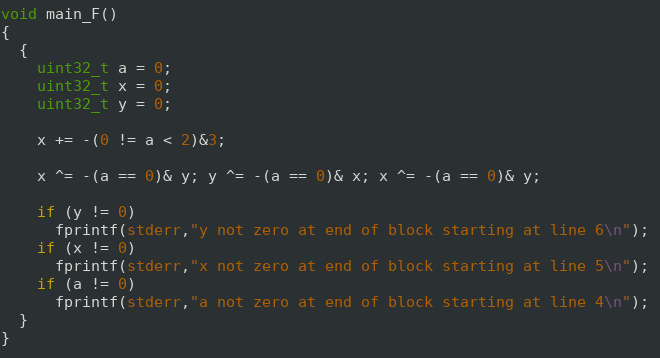
\includegraphics[width=0.9\textwidth]{conditionals_c.png}
        \caption{Conditionals translated to C}
        \label{fig:conditionals_c}
    \end{minipage}
\end{figure}

% Hermes has const arrays now
\subsection{Constants}
Hermes allows for constant values to be declared. These are not required to be 0 at the end of a function and are initialized with a value other than 0. However, it was only singleton values that were allowed to use the const keyword so I added the ability to specify constant arrays of varying sizes. This was done by adding an entry for it in the AST, the Compiler and the typesystem.
%(* TODO: I also added out of bounds checks *)

Being able to define const arrays is very useful for algorithms such as Twofish that have large 16x16 arrays. In the past, populating large arrays was done through a call to a function that would add values to all the entries of the array. Now it can be done directly in the function that uses it.

\section{The algorithm}
In 1972 and 1974, the National Bureau of Standards (now the National Institute of Standards and Technology, or NIST) issued the first public request for an encryption standard. The result was DES \cite{NBS77}, arguably the most widely used and successful encryption algorithm in the world. However, due to advances in distributed key search techniques, the key was found to be too short for modern security applications.
Triple-DES emerged as a temporary solution in many high-security applications, such as banking, but it was too slow for some uses. More fundamentally, the 64-bit block length shared by DES and most other well-known ciphers opens it up to attacks when large amounts of data are encrypted under the same key.

Twenty years later, in 1997, NIST announced the Advanced Encryption Standard (AES) \cite{NIST97a}. NIST requested comments from the public on the proposed standard, and eventually issued a call for algorithms to satisfy the standard \cite{NIST97b}. NIST made all submissions public and eventually, through a process of public review and comment, chose a new encryption standard to replace DES. Twofish did not win, but made it as one of the five finalists in the 1997 competition.

Twofish is a 16 byte / 128-bit block cipher with a variable key length between 128 and 256 bits. The cipher is a 16-round Feistel network also called a substitute-permute network. It has a bijective function F consisting of four key-dependent 8-by-8-bit S-boxes (Substitution-boxes) \cite{wiki_sbox}, a fixed 4-by-4 MDS (maximum distance separable) matrix over GF($2^8$) (Galois-field), a PHT (pseudo-Hadamard transform), bitwise rotations, and a carefully designed key schedule.

I will go over each of these building blocks, explaining what they are:

\subsection{Feistel Networks}
A Feistel network is a general method of transforming any function (usually called the F function) into a permutation. It was invented by Horst Feistel in 1973.

The fundamental building block of a Feistel network is the F function: a key-dependent mapping of an input string onto an output string. An F function is always non-linear and possibly non-surjective\footnote{A non-surjective F function is one in which not all outputs in the output space can occur.}:

\begin{equation*}
  F : \lbrace 0, 1\rbrace^{n/2} x \lbrace0, 1\rbrace^N -> \lbrace 0, 1\rbrace^{n/2}
\end{equation*}

where n is the block size of the Feistel Network, and F is a function taking n/2 bits of the block and N bits of a key as input, and producing an output of length n/2 bits. In each round, the “source block” is the input to F , and the output of F is XOR'ed with the “target block,” after which these two blocks swap places for the next round. The idea here is to take an F function, which may be a weak encryption algorithm when taken by itself, and repeatedly iterate it to create a strong encryption algorithm.  Two rounds of a Feistel network is called a \textbf{cycle}. In one cycle, every bit of the text block has been modified once.

\subsection{S-boxes}
An S-box is a table-driven non-linear substitution operation used in most block ciphers. S-boxes vary in both input size and output size, and can be created either randomly or algorithmically. S-boxes were first used in Lucifer by Horst Feistel, then DES, and afterwards in most encryption algorithms. Twofish uses four different, bijective, key-dependent, 8-by-8-bit S-boxes. These S-boxes are built using two fixed 8-by-8-bit permutations and key material.

\subsection{A small example}
Lets talk a little bit about the magic of substitute-permute networks. As the name implies, we first do a substitution followed by a permutation. I'll give a small example with a 2-by-2-bit S-box followed by a substitution.
Lets say you have a table of substitutions. 2 bits means we have 4 different values '00', '01', '10' and '11'.
So we do a mapping which could look like this:
\begin{table}[h!]
  \begin{center}
    \label{fig:small_subs_example}
    \begin{tabular}{|c|c|c|c|}
      \hline
      00 & 01 & 10 & 11 \\ \hline
      10 & 00 & 11 & 01 \\ \hline
    \end{tabular}
    \caption{2-by-2-bit S-box example.}
  \end{center}
\end{table}

This means that if we see '10' we substitute it to '11' and if we see '11' we substitute it to '01'. Thats the substitution part. \\
For the permutation part, lets say we have two of these 2-bit S-boxes. The output would be 2 bits from each, so we have 4 bits of output in total. The permutation is switching bits like this:
(* Insert permutation picture *)
%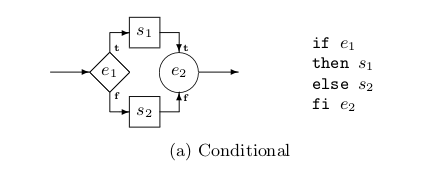
\includegraphics{permutation_example.png}[scale=0.7] \\
So if we want to substitute-permute the number 4 for example it would look like '0100', so the first Sbox would have input '01' and the second Sbox would have input '00'. This would result in the output of the first S-box being '00' and the output of the second S-box to be '10'. So the number 4 goes through the two S-boxes and comes out as a 2. Then it enters the permutation and becomes TODO:

This constitutes one round of encryption. Now obviously this process is very easy to reverse if the substition table and the permutation table are public, so that is why we mix in keys. We XOR before the first encryption (input whitening), we XOR after each round and we XOR again after the last round (output whitening). Once you take the key away you can no longer reverse the process.

Twofish uses 16 rounds and AES uses 10-14 rounds. The tradeoff here is obviously speed. If you use too few rounds the encryption will be easier to break, but if you use too many it will be slow.


\subsection{MDS Matrices}
An MDS matrix is a linear mapping from a field elements to b field elements. It produces a composite vector of a + b elements with the property that for each non-zero vector there will be atleast b + 1 non-zero elements.
What this means is that the "distance" between two distinct vectors produced by the MDS mapping is atleast b + 1.
It is provable that no mapping can have a larger minimum distance between two distinct vectors and that is why we call it maximum distance seperable.
Twofish uses a 4-by-4 MDS matrix over GF ($2^8$) called the Reed-Solomon (RS) error-correcting codes.

\subsection{Pseudo-Hadamard transforms}
The 32-bit pseudo-Hadamard transform (PHT) that Twofish uses is a mixing operation that given two inputs a and b updates the two values as follows:
%\begin{equation*}
%  a' = a + b mod 2^{32} \\
%  b' = a + 2b mod 2^{32}
%\end{equation*}

\subsection{Whitening}
Input/output whitening is done by XOR'ing 128 bits of subkey, which is not used in any of the rounds, with part of the expanded key before the first round and after the last round. It was shown in 1996 by Rivest \cite{KR96} that whitening made it substantially harder for attackers to do keysearch attacks.

\subsection{Key schedule}
The key schedule is the means by which the key bits are turned into round keys that the cipher can use.  Twofish needs a lot of key material, and has a complicated key schedule. To facilitate analysis, the key schedule uses the same primitives as the round function.

There are two types of keys used for the twofish algorithm. It uses a user-supplied global key M of 128 bits to generate two sets of subkeys S and K. S has two subkeys $S_0$ and $S_1$ which are fixed during the entire encryption and decryption process. $S_0$ and $S_1$ are used in the S-boxes inside the g function. The key schedule performs a key expansion to make K, which is a 40-word expanded key where each word consists of 32 bits. I'll refer to these as $K_0$ through $K_{40}$. Words 0-7 are used for input / output whitening whilst the remaining 32 words are passed on to the bijective function F two at a time during the 16 rounds of encryption. \\

The generation of S is done by multiplication in the Galois field GF $(2^8)$ where the primitive polynomial is $x^8 + x^6 + x^3 + x^2 + 1$.

TODO: I have not implemented key schedule as there is a problem with galois field multiplication when b == 0 which happens in the key schedule.
%\begin{lstlisting}
% This is what we want if we use key schedule
%     __       _____
%0 - |ks| --  |ks^-1| - 0
%k - |__| --  |____ | - k
%          |
%          |
%   d  ---enc ---- c
%\end{lstlisting}



% Baggrund om side channel vulnerabilities og ARM64
\chapter{Side-channel Vulnerabilities}
\label{chapt - Side-channel}
\section{Side-channel Vulnerabilities}
Executing a computation on an electronic device consumes time and power, radiates an electromagnetic field, dissipates heat and even makes some noise\cite{Gnad_Krautter_Tahoori_2019}. 
Side-channel attacks aim to take advantage of these leakages, by measuring these physically observable phenomenons; instead of perceiving the cryptographic primitive as a software black box (some transformation that, given some secret parameter, turns some input into output), these new types of attacks target the \emph{environment} such as the process, the processor, the RAM etc. instead of the actual algorithm.

If an adversary is able to extract bits of knowledge about the environment through analysis of running time, power consumption, electromagnetic radiation etc., she may be able to recover the secret parameters involved in the computation.



\subsection{Examples}
\subsubsection{Row hammer attack}
\begin{wrapfigure}{r}{0.4\textwidth}
  \begin{center}
    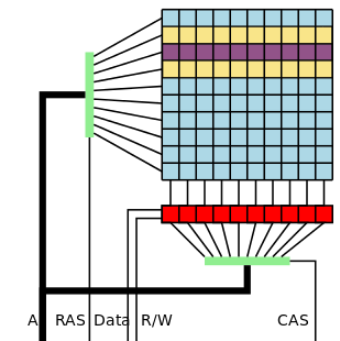
\includegraphics[width=0.3\textwidth]{rowhammer_vis.png}
  \end{center}
  \caption{Rapid row activations (yellow rows) may change the values of bits stored in victim row (purple row).}
\end{wrapfigure}

In 2015, Project Zero, a team of security analysts employed by Google tasked with finding zero-day vulnerabilities, disclosed an attack they named Rowhammer, that would allow for bit flips in a system.
Because newer DRAM has such a high cell density, millions of repeated accesses per second (i.e. hammering) on rows of cells of memory can lead to bit flips in neighboring rows.
A rowhammer attack bypasses memory protection, as one process can affect others, making it very hard to defend against.

%An example of a rowhammer attack is shown in figure \ref{fig:rowhammer_x86} where an attacker repeatedly reads two values, bypassing the cache.
%
%\begin{wrapfigure}{r}{0.4\textwidth}
%  \begin{center}
%    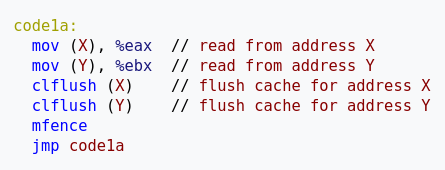
\includegraphics[width=0.4\textwidth]{rowhammer_x86.png}
%  \end{center}
%  \caption[caption]{Small x86-snippet that induces the row hammer effect\hspace{\textwidth} From Blackhat2015 talk [CITE: Blackhat2015\_rowhammer]}
%  \label{fig:rowhammer_x86}
%\end{wrapfigure}

Attacks from the Rowhammer-family, such as Throwhammer, RAMBleed and NetCAT, that perform read/write on memory have since been shown to cause all kinds of havoc from privilege escalation to keylogging to breaking cryptographic keys\cite{tatar_throwhammer:_2018}\cite{kwong2020rambleed}\cite{kurth_netcat:_2020}.
It is worth mentioning, however, that side-channel attacks are highly implementation-specific and thus much harder to generalize than if you were to break the algorithm.

\subsubsection{Cold boot attacks}
In 2008, a research paper on cold boot attacks\cite{Halderman2008LestKeys} was published from Princeton University. By physically freezing the memory, attackers were able to read data from the DRAM up to several minutes after cutting power to the victim machine. Cutting power to the victim computer leaves it with no chance to erase its sensitive data from memory. From there an attacker can either restore power and launch a custom kernel leaving a small memory footprint, or transplant the DRAM modules to another computer keeping the DRAM completely intact.

In theory, Hermes is vulnerable to cold boot attacks. In practice, however, it would be near impossible simply because Hermes clears memory after it has run so the power would have to be cut at the exact time where the sensitive data is used. Another property Hermes has, that makes it really difficult to do cold boot attacks is the fact that Hermes uses pass-by-reference. Values are easily corrupted and inline updates are frequent.

\subsubsection{Simple Power Analysis}
Simple Power Analysis (SPA), which is one of two main power consumption analysis methods, focuses on the \emph{operations} that have taken place can tell an attacker a lot about what encryption algorithm is being used.
For example, 10 similar operations in a row can indicate that the algorihtm is AES due to its ten rounds of encryption. 16 rounds could indicate it may be Twofish etc.

This is a very effective method of analysis if the instruction flow depends on the data. 
Modular exponentiation is an example of this: if the square operation is implemented differently than the multiply, (which is a tempting choice since it can be optimized for running time) then the powertrace of an exponentiation directly yields the exponents value.
The following figure shows how SPA has been used to cryptanalyze an RSA algorithm:
\begin{figure}[htp]
  \begin{center}
    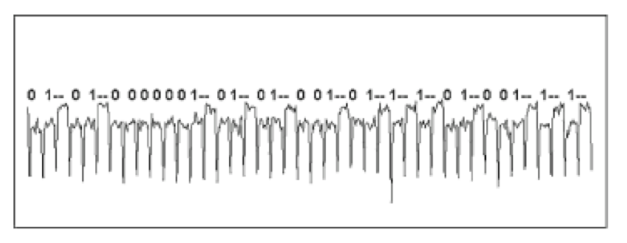
\includegraphics[scale=0.5]{SPA_leaks_from_RSA_implementation.png} \\
  \end{center}
  \caption[caption]{SPA leaks from an RSA implementation. \hspace{\textwidth} From Introduction to Differential Power Analysis \cite{KOCHER2011}}
\end{figure}

%Differential Power Analysis (DPA) takes multiple traces of two sets of data, then computes the difference of the averages. Given enough traces, even tiny correlations can be seen, regardless of how much noise is in the system, since it will effectively cancel out during the averaging.


\subsection{Classifying attacks}
Attacks are often classified along two axes falling into one of four categories: \cite{FX2010}.

\begin{itemize}
  \item \textbf{Hardware tampering}
    \begin{itemize}
      \item[1.] Invasive - Attacks which try to read the actual data either by intercepting or directly reading data. An example of this could be to connect a wire onto the data bus and view the data transfers or doing some sort of memory inspection.
      \item[2.] Non-invasive - Attacks which do not read the actual data, but exploits externally available information. External information can be observations on running time, power consumption and such.
    \end{itemize}
  \item \textbf{System tampering}
    \begin{itemize}
      \item[3.] Active - Attacks that tries to change the behaviour of some function on the device, such as introducing a fault in the computation to cause a leak of information, or cold-booting the device to perform memory dumps \cite{Halderman2008LestKeys}.
      \item[4.] Passive - Attacks that only observes a devices behaviour, without affecting it. No signs of compromise or failure.
    \end{itemize}
\end{itemize}

Figure \ref{fig:sca_classification} visualizes these classifications with hardware tampering along the x axis and system tampering along the y axis.
The safety that Hermes intends to provide is against timing attacks and information leakage which includes cold boot attacks.
Timing attacks are non-invasive and passive as the attacker only observes the running time of the process.
Cold boot attacks are active attacks as they perform memory dumps, but can be either invasive or non-invasive exemplified in \cite{Halderman2008LestKeys} where, in one attack, researchers freeze the chip thereby tampering with the hardware.

\begin{figure}[h!]
  \resizebox{0.9\columnwidth}{!}{%
      \begin{tikzpicture}
        \draw [thick] (0,5) node (yaxis) [above] {Active}
          |- (0,-5) node (yaxis) [below] {Passive}
          |- (5,0) node (xaxis) [right] {Invasive}
          |- (-5,0) node (xaxis) [left] {Non-invasive};
        \node[draw, fill=green] at (-4,4) {Cold Boot Attack};
        \node[draw, fill=green] at (4,4) {Cold Boot Attack};
        \node[draw, fill=red] at (-4,-3) {Power analysis};
        \node[draw, fill=green] at (-4,-4) {Timing Attack};
        \node[draw, fill=red] at (4,3) {Row hammer};
        \node[draw, fill=red] at (4,2) {RAMBleed};
        % Legend
        \matrix [draw, below left] at (6,-3.5) {
          \node [fill=green] {Protection\ \ \ \ \ \ \ }; \\
          \node [fill=red] {No Protection}; \\
        }; 
      \end{tikzpicture}%
  }
  \caption{Some side-channel attacks and their classifications} 
  \label{fig:sca_classification}
\end{figure}

\clearpage
\newpage

Side-channels attacks have been gaining a lot of attention recently by device manufactorers. Especially the non-invasive, passive attacks which are hard to spot and can generally be performed using relatively cheap equipment.


\chapter{RSSA}
\input{Sections/Hermes_To_RSSA/intro.tex}
\section{ARM Grammar}


%Prior to this thesis Hermes only allowed constant declarations to be variables, but for Twofish it was really useful to extend this to allow constant matrix declarations as well. A ConstArrayDecl in the abstract syntax tree has the type \b{string * string * string list * typ * pos} which is name, size, elements, type and position.

%I første omgang laver den det til RSSA men hvor variablene er tupler af (var og int option) som er deres subscript. En slags RIL form.
%Dernæst laver den det til RSSA ved at give variablene indekser.
%
%Eksempel på for-loop oversættelse:
%plus5 (u32 x) {
%  for (i = 0; 3) {
%    x += 5;
%  }
%}
%
%entry; loop <- i == 0 betyder hvis i == 0 kommer vi fra entry ellers fra loop
%
%begin plus5
%i += 0
%-> entry
%entry; loop <- i == 0
%x += 5
%i += 1
%i < 3 -> loop; exit
%exit <-
%end plus5
%
%skal bruge: 
%* labelnavn for unik loop label
%* 2x variabel from og to
%* instruktionsliste der skal eksekveres
%* pos
%
%
%Eksempel på if oversættelse
%if5 (u32 x) {
%  u32 y;
%  if (x == 5) {
%    y += 3;
%  }
%}
%
%begin if5
%x == 5 -> true; skip
%true <-
%y += 3
%-> exit
%x == 5 <- exit; skip
%end if5
%
%skal bruge:
%* labelnavn for unik if label
%* if condition (exp)
%* rssa\_instr (måske list?) som skal udføres i body
%\section{RSSA AST}
%array er nødt til at have en expression som index tror jeg?
%MemUpdate skal tage et array med et index 
%(* TODO: GRAMMAR *)

%\section{RSSA compiler}
%Update:
%Det svære ved update er, at vi kan have arbitrært nestede expressions og vi er på single assignment.
%Dvs. vi skal have compilet det nestede expression og ende med at resultatet er i en variabel vi har navnet på.
%Derfor opretter vi først en tmp variabel, dernæst compiler vi expressionen, og i vores in klausul har vi først alle opdateringerne (som ender med at lægge en værdi i tmp), og dernæst en RSSA.Assign/MemUpdate som tager s (som skal have nyt indeks i næste skridt RIL -> RSSA hvis det er en Assign) og bruger updateop så det bliver (s, NONE) updateOp tmp.
%
%
%
%Inc:
%Vi bruger RSSA.Assign/MemUpdate på det vi vil opdatere med makeConst "1" og Hermes.Plus som binOp.
%
%Dec:
%Samme som inc bare med Hermes.Minus
%
%Compiler local decls som en string
%Mange steder hvor tabellen 1 bruger vars men vi bruger var\_idxs. Kun første gang man bruger var.


\chapter{ARM64}
\section{ARM}
ARM64 or AArch64 is a family of reduced instruction set computing (RISC) architectures developed by Arm Holdings.
It is currently the most widely used instruction set architecture with more than 100 billion ARM processors produced as of 2017\cite{ARM_sales}. 
ARM is used in many applications, such as Raspberry Pis, self driving cars, phones, tablets etc. Apple, who has been using ARM in their iPhones and iPads recently announced they will be switching from x86 to ARM on their MacBooks from 2020 and onwards\cite{ARM_cpus_2020}.

\subsection{ARM64 vs x86\_64}
% Addressing modes such as load unsigned byte
% Segment registers (CS: code segment, DS: data segment, SS: stack segment, ES: extra segment, FS, GS)
% x86 has variable-length instructions, while ARM is always 32 bit.
% Macro instructions such as ...
% Thumb modes for ARM ...
% CITE [http://www.informit.com/articles/article.aspx?p=1620207&seqNum=3]
Because ARM has a reduced instruction set, it is generally cheaper, less power consuming and dissipates less heat than complex instruction set computing (CISC) architectures such as x86, designed by Intel in the early 80s. This makes it a really great choice for smartphones, laptops and IOT devices.
ARM architectures have fewer instructions available than x86. However x86 has a lot of legacy aspects such as addressing modes and segment registers that are rarely used as well as macro instructions, which can contain several instructions in one and take more work to decode. As a result of this, the ARM pipelines are generally much shorter ranging from 3 to 8 stages compared to that of x86's 14 to 32 stages.

x86 has variable-length instruction support, whereas the ARM instruction decoder always takes a 32-bit word and just needs to test a few bits to know where to dispatch the instruction. The x86 decoder needs to read the bits in sequence, find breaks between instructions, and so on.  
In general x86 processors are more powerful and a better choice for projects that require complex displays such as gaming or animation, but also require a heat sink i.e. somewhere to dump their heat dissipation. A high-end Intel i7 processor can consume as much as 130W of power, whereas ARM cores typical power consumption is approximately 5W.

ARM64 is a natural choice for Hermes since our focus is to protect small devices.

\section{ARM Grammar}


\section{RSSA To ARM64}

\section{ARM Compiler}


% Afsnit om min twofish implementation med referencer til twofish bogen
\chapter{Hermes implementation of Twofish}
\label{chapt - Hermes implementation}
\section{Reversible Twofish}
\subsection{Reference implementation}
Bruce Schneier, who is a co-author of the algorithm, has a Github repository \cite{Git2F} with two implementations of Twofish: A highly optimized one in C and another one in Python2.7.
I will be focusing on the Python implementation as it is more similar to the Hermes implementation in its structure as well as being easier to read.
Its around 250 lines of code, so not awfully large but not small either. The complexity of the code is low/medium and it is overall pretty straight forward if you know how the algorithm works.

TODO: Snak om lifting scheme + konkluder hvorvidt Hermes er passende som domænespecifikt krypteringssprog

\subsection{encrypt/decrypt}
\subsubsection{Python}
Lets look at the encrypt/decrypt definitions.
\lstinputlisting[label=app:Encrypt Python,caption=encrypt/decrypt in Python, language=Python,frame=single] {"Listings/encrypt.py"}
We see that the only difference between encrypt and decrypt is the order in which they do things.
Encrypt uses the words K[0]-K[3] for input whitening, calls F 16 times with roundnumber r = 0 to 16, and then performs output whitening with the words K[4]-K[7]. Decrypt does the same but in the other direction. 

The parameters for the functions are subkeys K and S as well as a plaintext/ciphertext.
They both call F with five arguments: input words R[0] and R[1], the round number r which is used to select which subkeys to use, and the subkeys K and S.

\subsubsection{Hermes}
My implementation is structurally similar to the Python version. Lets have a look:
\lstinputlisting[label=app:Encrypt Hermes,caption=encrypt in Hermes, language=Hermes,frame=single] {"Listings/encrypt.hms"}
Here we see the same structure; input whitening followed by 16 rounds of encryption followed by output whitening. It has the same logic (calling F and rotating/XOR'ing) as the Python implementation. TODO: It uses Bennetts method of passing along some placeholder variables that can store some intermediate values which we can use to reset the inplace updated variables later with uncall.

\subsection{Galois Field multiplication}
Lorem ipsum..
%TODO: Galois Field multiplication is interesting because

\subsubsection{Python}
\lstinputlisting[label=app:GaloisField Python,caption=Galois Field multiplication in Python, language=Python,frame=single] {"Listings/gfmult.py"}

\subsubsection{Hermes}
%TODO: Det her må ku gøres pænere med flags array
%TODO: Polymult bruger Bennet? Snak om B ikke må være 0. Burde aldrig ske siger michael.
%TODO: GFMult er som sådan en reversibel funktion siger michael og den optræder i RSA. Konkluder evt. noget med at det her er babysteps towards en RSA implementation?
\lstinputlisting[label=app:GaloisField Hermes,caption=Galois Field multiplication in Hermes, language=Hermes,frame=single] {"Listings/gfmult.hms"}


% Kør min implementation af twofish 50 gange imod deres 50 gange
\chapter{Benchmarks}
\label{chapt - Benchmarks}
% Simple eksempler som jeg går i detaljer med
\section{Compilation}
test 

\section{Correctness}
test2

\section{Twofish}
test3



\chapter{Conclusions}
\label{chapt - Conclusion}
I've shown that Hermes is well suited to higher complexity encryption algorithms involving lifting schemes and Galois Field multiplications.


% Man kunne helt gak skrive noget om kvantecomputere her - nej det går ikke
% Kunne måske også nævne noget om Rust oversættelse
Property based testing af Twofish ala det Simon brugte
Biblioteker til GFMult så vi kan komme i mål med RSA og keySched til Twofish


% Til diskussionen kan man nævne Iodine: verifying constant-time execution of hardware artiklen?




% Referencer
\newpage
\renewcommand\bibname{References}
\bibliographystyle{plainurl}
\bibliography{references}
SSA afsnit i Modern compiler implementation in ML af Andrew w. Appel

% Appendices
\clearpage
\newpage
\begin{appendices}
\renewcommand*{\lstlistingname}{Appendix}
\chapter{Appendices}
\section{TEA Hermes Implementation}
\label{code:TEA_Full_Imp}
\lstinputlisting[label=app:TEA hermes,caption=TEA in hermes, language=Hermes,frame=single] {"Listings/tinyCrypt.hms"}
\newpage
\section{RC5 Hermes Implementation}
\label{code:RC5_Full_Imp}
\lstinputlisting[label=app:encryption hms, caption=RC5 encryption, language=Hermes,frame=single] {"Listings/rc5.hms"}

\end{appendices}

\end{document}
